
\documentclass[11pt]{book}

\usepackage{graphicx}
\usepackage{fancyhdr}
\usepackage{lipsum}
\usepackage[dvipsnames]{xcolor}
\usepackage{multicol} 
\usepackage[top=1in, bottom=1.25in, left=1.5cm, right=1.5cm]{geometry}
\usepackage{float}
\usepackage{titlesec, blindtext}
\usepackage{caption}
\usepackage{ifthen}
\usepackage{eso-pic} 
\usepackage[font=footnotesize,labelfont=bf]{caption}
\captionsetup{justification=raggedleft,singlelinecheck=false}

% no Intendation
\setlength{\parindent}{0pt}

\titlespacing\chapter{0pt}{12pt plus 4pt minus 2pt}{8pt plus 2pt minus 2pt}

\titleformat{\chapter}[display]
  {\normalfont\bfseries\huge\bfseries\color{Bittersweet}}{}{-100pt}{\Huge}

\setlength{\columnsep}{1cm}


\usepackage{fancyhdr}             % put things headers and footers and we plan misuse it ;)
\usepackage{lipsum}               % for sample text



\begin{document}

% Fitis %%%%%%%%%%%%%



\chapter{Fitis, \itshape Phylloscopus trochilus}

\textbf{Algemene Broedvogel} 
\vspace{5mm} %5mm vertical space



 \begin{figure}[H]
 \caption*{Bron: Waarnemingen.be}   
  \vspace{-1.2em}
  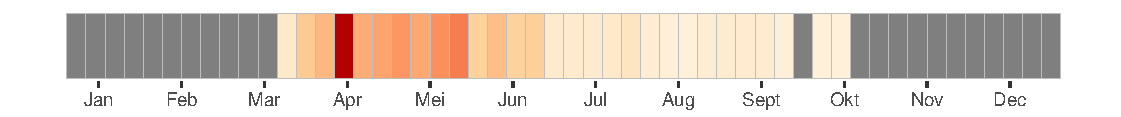
\includegraphics{Kalender/Fitis.pdf}
  \end{figure}

\begin{multicols}{2}

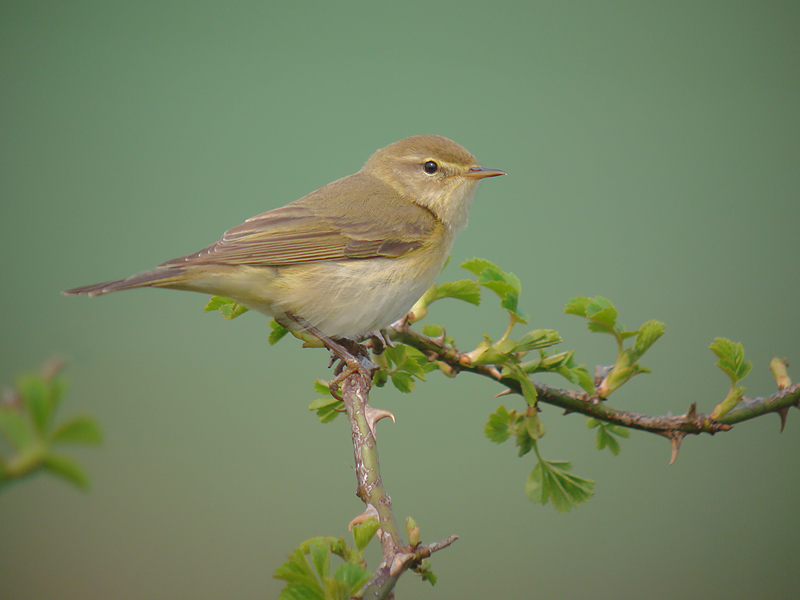
\includegraphics[width=8cm]{Foto's/Fitis.jpg}
\section{Bespreking}
\lipsum[1-2]
  \begin{figure}[H]
  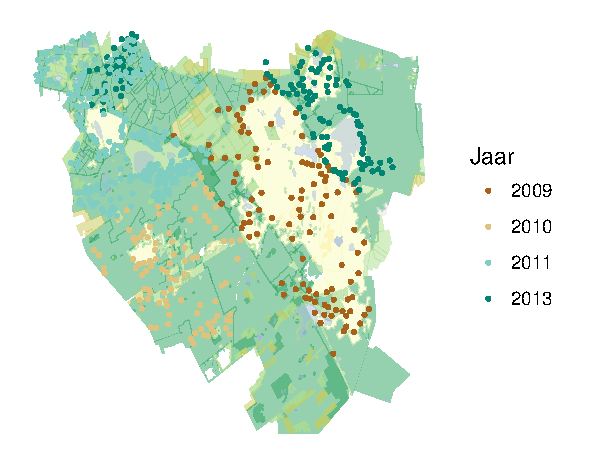
\includegraphics{Grenspark/Fitis.pdf}
  \vspace{-1.2em}
   \caption*{Bron: Broedvogelmonitoring Grenspark}   
  \end{figure}
  
\lipsum[1]

 \begin{figure}[H]
  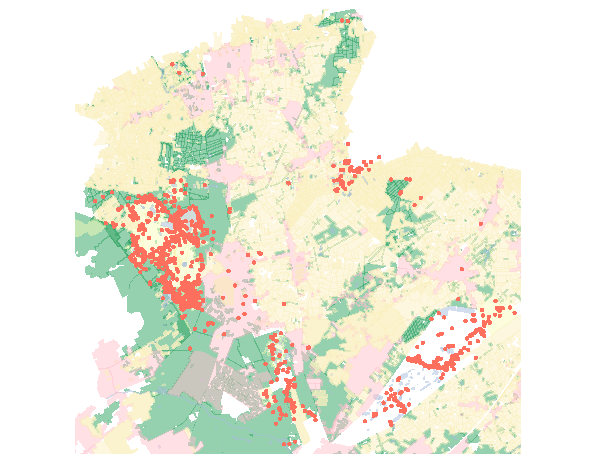
\includegraphics{Waarnemingen/Fitis.pdf}
  \end{figure}

 \begin{figure}[H]
  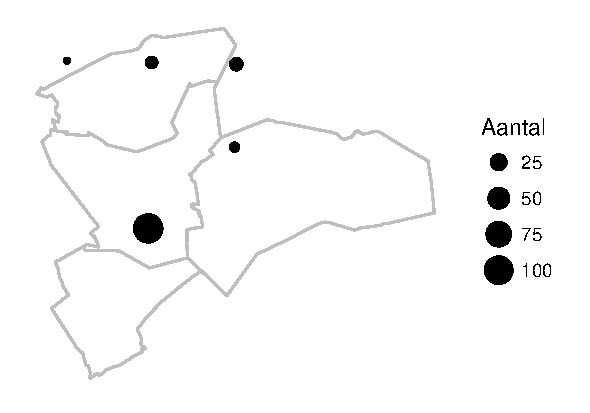
\includegraphics{Atlas/Fitis.pdf}
  \end{figure}
  
\lipsum[1]

\end{multicols}

\chapter{Bergeend, \itshape Tadorna tadorna}


\textbf{Zeldzame Broedvogel} 
\vspace{5mm} %5mm vertical space

 \begin{figure}[H]
  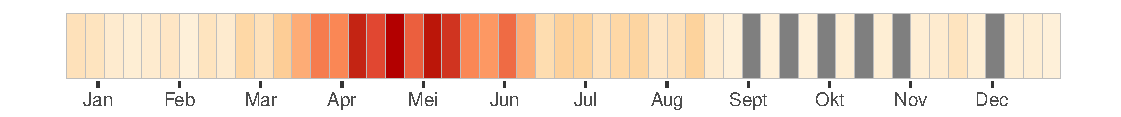
\includegraphics{Kalender/Bergeend.pdf}
  \end{figure}

\begin{multicols}{2}

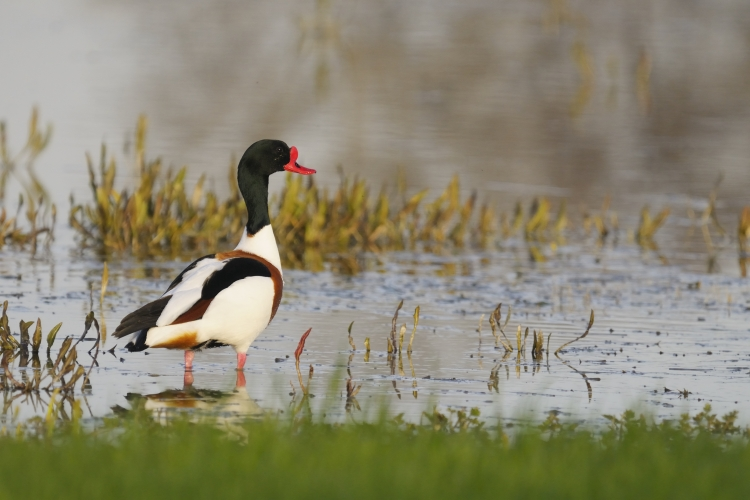
\includegraphics[width=8cm]{Foto's/Bergeend.jpg}
\section{Bespreking}

\lipsum[1-2]


  \begin{figure}[H]
  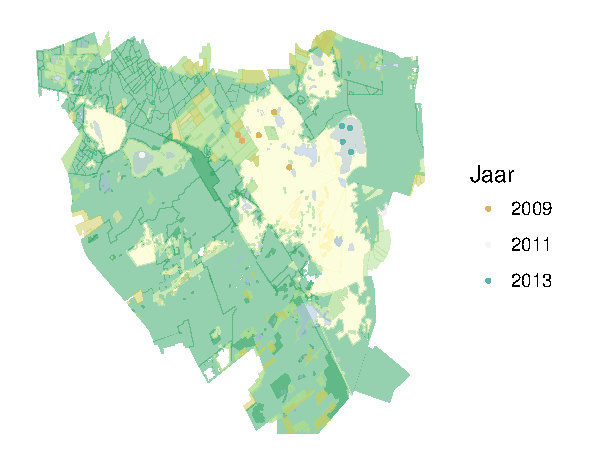
\includegraphics{Grenspark/Bergeend.pdf}
  \end{figure}
  
  
\lipsum[1]

 \begin{figure}[H]
  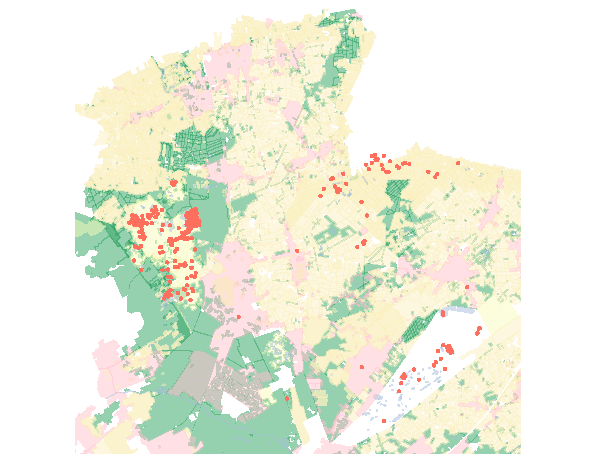
\includegraphics{Waarnemingen/Bergeend.pdf}
  \end{figure}
  
 \begin{figure}[H]
  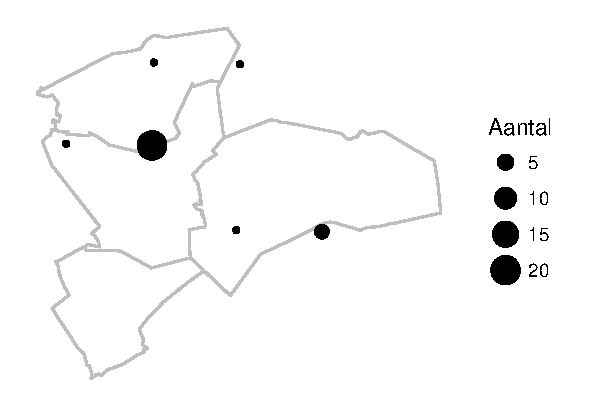
\includegraphics{Atlas/Bergeend.pdf}
  \end{figure}
  
\lipsum[1]

\end{multicols}



\chapter{Bosruiter, \itshape Tadorna tadorna}


\textbf{Vrij Algemene Doortrekker} 
\vspace{5mm} %5mm vertical space

 \begin{figure}[H]
  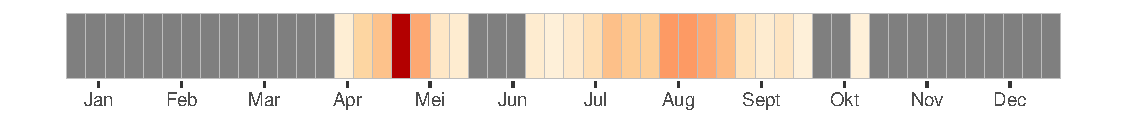
\includegraphics{Kalender/Bosruiter.pdf}
  \end{figure}

\begin{multicols}{2}

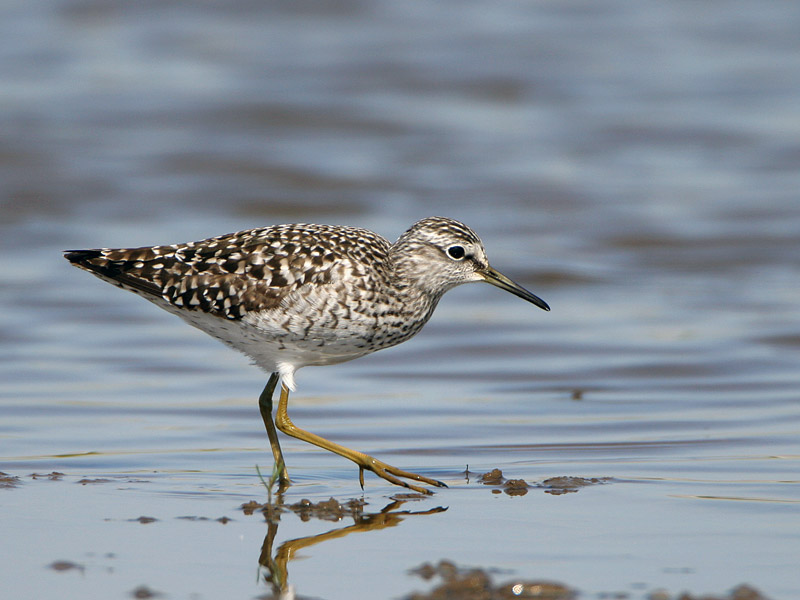
\includegraphics[width=8cm]{Foto's/Bosruiter.jpg}
\section{Bespreking}

\lipsum[1-2]


  \begin{figure}[H]
  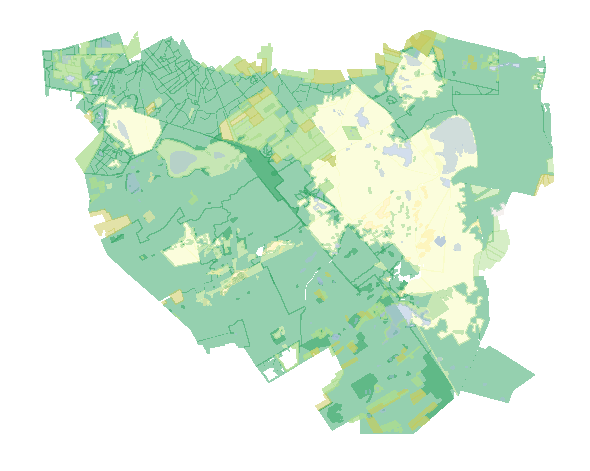
\includegraphics{Grenspark/Bosruiter.pdf}
  \end{figure}
  
  
\lipsum[1]


 \begin{figure}[H]
  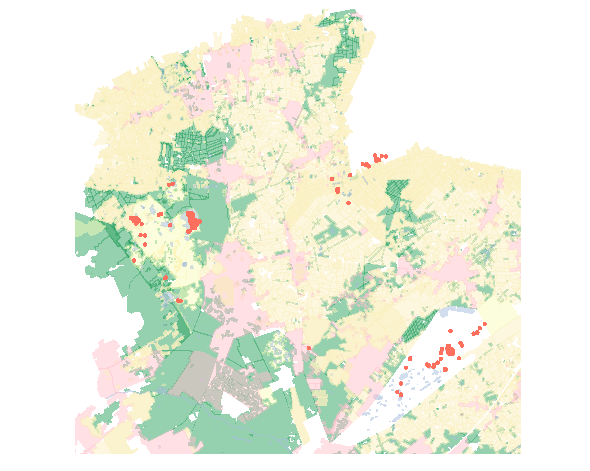
\includegraphics{Waarnemingen/Bosruiter.pdf}
  \end{figure}

 \begin{figure}[H]
  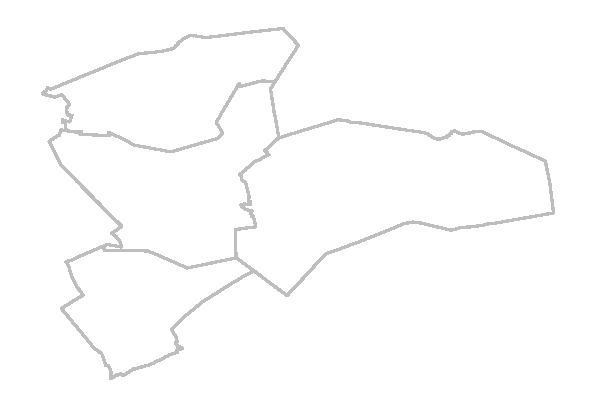
\includegraphics{Atlas/Bosruiter.pdf}
  \end{figure}
  
\lipsum[1]

\end{multicols}



\end{document}